\documentclass{article}
\usepackage{graphicx}
\usepackage{float}
\usepackage{listings}
\usepackage{color}
\usepackage{xcolor}
\usepackage{hyperref}
\usepackage{xepersian}

\settextfont{Yas} % You might need to upload a font like Yas.ttf or Tahoma.ttf to Overleaf
% Or use a font available on Overleaf's system if you don't upload one.
% For example: \settextfont{FreeFarsi} if available, or just upload a .ttf file.

\definecolor{codegreen}{rgb}{0,0.6,0}
\definecolor{codegray}{rgb}{0.5,0.5,0.5}
\definecolor{codepurple}{rgb}{0.58,0,0.82}
\definecolor{backcolour}{rgb}{0.95,0.95,0.92}

\lstdefinestyle{mystyle}{
    backgroundcolor=\color{backcolour},   
    commentstyle=\color{codegreen},
    keywordstyle=\color{magenta},
    numberstyle=\tiny\color{codegray},
    stringstyle=\color{codepurple},
    basicstyle=\ttfamily\footnotesize\setLTR,
    breakatwhitespace=false,         
    breaklines=true,                 
    captionpos=b,                    
    keepspaces=true,                 
    numbers=left,                    
    numbersep=5pt,                  
    showspaces=false,                
    showstringspaces=false,
    showtabs=false,                  
    tabsize=2
}
\lstset{style=mystyle}

\title{Breast Cancer Analysis with SHAP and LIME}
\author{Mina}
\date{\today}

\begin{document}

\maketitle
\tableofcontents
\newpage


\section{Breast Cancer Diagnosis Analysis

This notebook loads the WDBC dataset, trains a Random Forest classifier to predict diagnosis (Malignant vs Benign), and interprets the model using SHAP and LIME.}


\begin{latin}
\begin{lstlisting}[language=Python]
import pandas as pd
import numpy as np
import matplotlib.pyplot as plt
import seaborn as sns
from sklearn.model_selection import train_test_split
from sklearn.ensemble import RandomForestClassifier
from sklearn.metrics import accuracy_score, classification_report, confusion_matrix
from sklearn.preprocessing import LabelEncoder
import shap
import lime
import lime.lime_tabular

# Set plot style
sns.set(style="whitegrid")
\end{lstlisting}
\end{latin}

#\section{1. Load Data
Loading the dataset and assigning column names based on `wdbc.names`.


\begin{latin}
\begin{lstlisting}[language=Python]
# Define column names
features_mean = ['radius_mean', 'texture_mean', 'perimeter_mean', 'area_mean', 'smoothness_mean', 'compactness_mean', 'concavity_mean', 'concave_points_mean', 'symmetry_mean', 'fractal_dimension_mean']
features_se = ['radius_se', 'texture_se', 'perimeter_se', 'area_se', 'smoothness_se', 'compactness_se', 'concavity_se', 'concave_points_se', 'symmetry_se', 'fractal_dimension_se']
features_worst = ['radius_worst', 'texture_worst', 'perimeter_worst', 'area_worst', 'smoothness_worst', 'compactness_worst', 'concavity_worst', 'concave_points_worst', 'symmetry_worst', 'fractal_dimension_worst']

columns = ['ID', 'Diagnosis'] + features_mean + features_se + features_worst

# Load data
df = pd.read_csv('wdbc.data', names=columns, header=None)

# Display first few rows
df.head()
\end{lstlisting}
\end{latin}

\begin{latin}
\begin{verbatim}
         ID Diagnosis  radius_mean  texture_mean  perimeter_mean  area_mean  \
0    842302         M        17.99         10.38          122.80     1001.0   
1    842517         M        20.57         17.77          132.90     1326.0   
2  84300903         M        19.69         21.25          130.00     1203.0   
3  84348301         M        11.42         20.38           77.58      386.1   
4  84358402         M        20.29         14.34          135.10     1297.0   

   smoothness_mean  compactness_mean  concavity_mean  concave_points_mean  \
0          0.11840           0.27760          0.3001              0.14710   
1          0.08474           0.07864          0.0869              0.07017   
2          0.10960           0.15990          0.1974              0.12790   
3          0.14250           0.28390          0.2414              0.10520   
4          0.10030           0.13280          0.1980              0.10430   

   ...  radius_worst  texture_worst  perimeter_worst  area_worst  \
0  ...         25.38          17.33           184.60      2019.0   
1  ...         24.99          23.41           158.80      1956.0   
2  ...         23.57          25.53           152.50      1709.0   
3  ...         14.91          26.50            98.87       567.7   
4  ...         22.54          16.67           152.20      1575.0   

   smoothness_worst  compactness_worst  concavity_worst  concave_points_worst  \
0            0.1622             0.6656           0.7119                0.2654   
1            0.1238             0.1866           0.2416                0.1860   
2            0.1444             0.4245           0.4504                0.2430   
3            0.2098             0.8663           0.6869                0.2575   
4            0.1374             0.2050           0.4000                0.1625   

   symmetry_worst  fractal_dimension_worst  
0          0.4601                  0.11890  
1          0.2750                  0.08902  
2          0.3613                  0.08758  
3          0.6638                  0.17300  
4          0.2364                  0.07678  

[5 rows x 32 columns]
\end{verbatim}
\end{latin}

#\section{2. Preprocessing
- Drop ID column
- Encode Diagnosis (M=1, B=0)
- Split into Train and Test sets


\begin{latin}
\begin{lstlisting}[language=Python]
# Drop ID column as it's not useful for prediction
df = df.drop('ID', axis=1)

# Encode Diagnosis: Malignant (M) -> 1, Benign (B) -> 0
le = LabelEncoder()
df['Diagnosis'] = le.fit_transform(df['Diagnosis'])

print("Class encoding:", dict(zip(le.classes_, le.transform(le.classes_))))

# Split features (X) and target (y)
X = df.drop('Diagnosis', axis=1)
y = df['Diagnosis']

# Train-test split (80-20)
X_train, X_test, y_train, y_test = train_test_split(X, y, test_size=0.2, random_state=42)

print(f"Training shape: {X_train.shape}")
print(f"Testing shape: {X_test.shape}")
\end{lstlisting}
\end{latin}

\begin{latin}
\begin{verbatim}
Class encoding: {'B': np.int64(0), 'M': np.int64(1)}
Training shape: (455, 30)
Testing shape: (114, 30)

\end{verbatim}
\end{latin}

#\section{3. Train Random Forest Model


\begin{latin}
\begin{lstlisting}[language=Python]
# Initialize and train Random Forest Classifier
rf_model = RandomForestClassifier(n_estimators=100, random_state=42)
rf_model.fit(X_train, y_train)

print("Model training complete.")
\end{lstlisting}
\end{latin}

\begin{latin}
\begin{verbatim}
Model training complete.

\end{verbatim}
\end{latin}

#\section{4. Evaluate Model


\begin{latin}
\begin{lstlisting}[language=Python]
# Predictions
y_pred = rf_model.predict(X_test)

# Evaluation
accuracy = accuracy_score(y_test, y_pred)
print(f"Accuracy: {accuracy:.4f}\n")

print("Classification Report:")
print(classification_report(y_test, y_pred, target_names=['Benign', 'Malignant']))

print("Confusion Matrix:")
cm = confusion_matrix(y_test, y_pred)
sns.heatmap(cm, annot=True, fmt='d', cmap='Blues', xticklabels=['Benign', 'Malignant'], yticklabels=['Benign', 'Malignant'])
plt.ylabel('Actual')
plt.xlabel('Predicted')
plt.title('Confusion Matrix')
plt.show()
\end{lstlisting}
\end{latin}

\begin{latin}
\begin{verbatim}
Accuracy: 0.9649

Classification Report:
              precision    recall  f1-score   support

      Benign       0.96      0.99      0.97        71
   Malignant       0.98      0.93      0.95        43

    accuracy                           0.96       114
   macro avg       0.97      0.96      0.96       114
weighted avg       0.97      0.96      0.96       114

Confusion Matrix:

\end{verbatim}
\end{latin}

\begin{figure}[H]
\centering
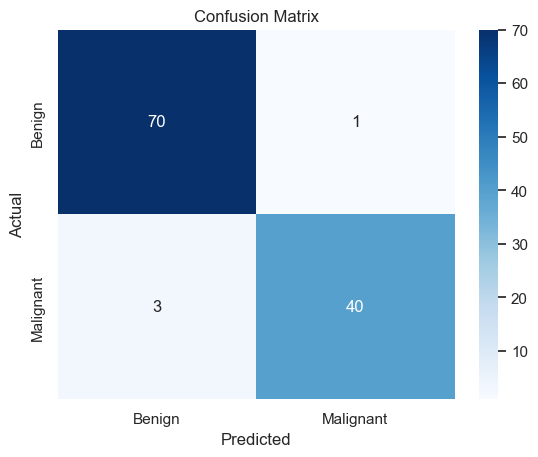
\includegraphics[width=0.8\textwidth]{images/img_0.png}
\caption{Output Image}
\end{figure}

#\section{5. SHAP Analysis
SHAP (SHapley Additive exPlanations) values explain the output of a machine learning model.


\begin{latin}
\begin{lstlisting}[language=Python]
# Initialize JS visualization code for SHAP
shap.initjs()

# Create object that can calculate shap values
# Using TreeExplainer which is optimized for Random Forests
explainer = shap.TreeExplainer(rf_model)

# Calculate Shap values
shap_values = explainer.shap_values(X_test)

# Summary Plot
print("SHAP Summary Plot (Feature Importance):")
shap.summary_plot(shap_values[:,:,1], X_test) # index 1 for the positive class (Malignant)
\end{lstlisting}
\end{latin}

\begin{latin}
\begin{verbatim}
<IPython.core.display.HTML object>
\end{verbatim}
\end{latin}

\begin{latin}
\begin{verbatim}
SHAP Summary Plot (Feature Importance):

\end{verbatim}
\end{latin}

\begin{figure}[H]
\centering
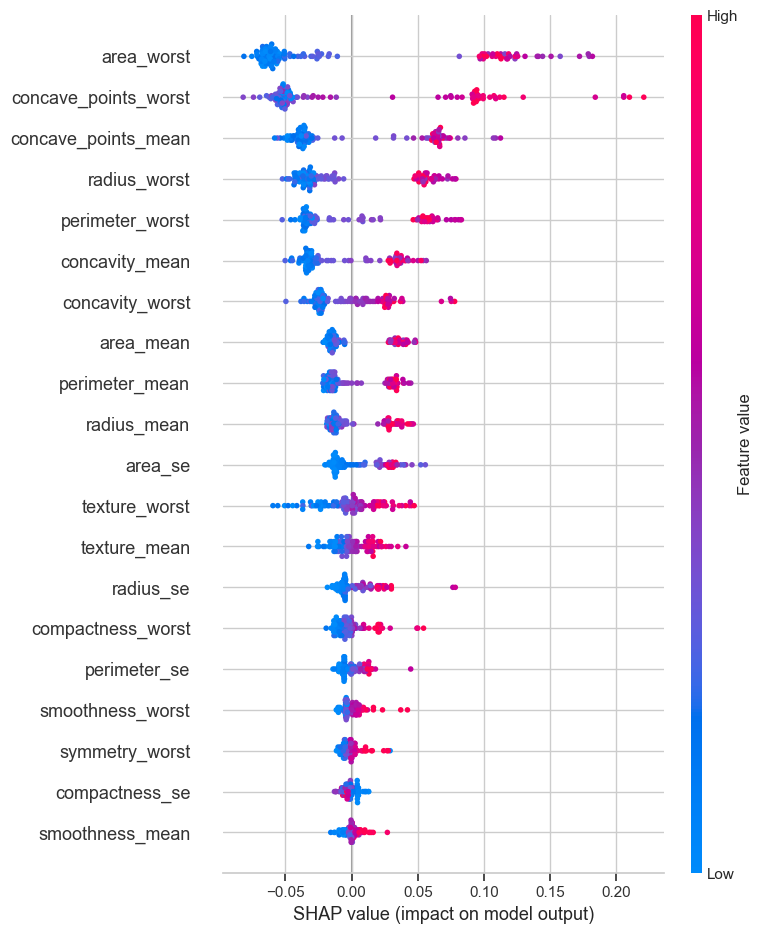
\includegraphics[width=0.8\textwidth]{images/img_1.png}
\caption{Output Image}
\end{figure}

#\section{6. LIME Analysis
LIME (Local Interpretable Model-agnostic Explanations) explains the predictions of any classifier.


\begin{latin}
\begin{lstlisting}[language=Python]
# Create a LIME explainer
lime_explainer = lime.lime_tabular.LimeTabularExplainer(
    training_data=np.array(X_train),
    feature_names=X_train.columns,
    class_names=['Benign', 'Malignant'],
    mode='classification'
)

# Pick a random instance from test set to explain
idx = 10 
instance = X_test.iloc[idx]
true_class = y_test.iloc[idx]

print(f"Explaining instance {idx}")
print(f"True Class: {'Malignant' if true_class == 1 else 'Benign'}")

# Generate explanation
exp = lime_explainer.explain_instance(
    data_row=instance,
    predict_fn=rf_model.predict_proba
)

# Show the explanation as a pyplot figure
fig = exp.as_pyplot_figure()
plt.show()
\end{lstlisting}
\end{latin}

\begin{latin}
\begin{verbatim}
Explaining instance 10
True Class: Benign

\end{verbatim}
\end{latin}

\begin{latin}
\begin{verbatim}
C:\Users\mina_\AppData\Local\Programs\Python\Python313\Lib\site-packages\lime\discretize.py:110: FutureWarning: Series.__getitem__ treating keys as positions is deprecated. In a future version, integer keys will always be treated as labels (consistent with DataFrame behavior). To access a value by position, use `ser.iloc[pos]`
  ret[feature] = int(self.lambdas[feature](ret[feature]))
C:\Users\mina_\AppData\Local\Programs\Python\Python313\Lib\site-packages\lime\discretize.py:110: FutureWarning: Series.__setitem__ treating keys as positions is deprecated. In a future version, integer keys will always be treated as labels (consistent with DataFrame behavior). To set a value by position, use `ser.iloc[pos] = value`
  ret[feature] = int(self.lambdas[feature](ret[feature]))
C:\Users\mina_\AppData\Local\Programs\Python\Python313\Lib\site-packages\lime\lime_tabular.py:544: FutureWarning: Series.__getitem__ treating keys as positions is deprecated. In a future version, integer keys will always be treated as labels (consistent with DataFrame behavior). To access a value by position, use `ser.iloc[pos]`
  binary_column = (inverse_column == first_row[column]).astype(int)
C:\Users\mina_\AppData\Local\Programs\Python\Python313\Lib\site-packages\sklearn\utils\validation.py:2749: UserWarning: X does not have valid feature names, but RandomForestClassifier was fitted with feature names
  warnings.warn(
C:\Users\mina_\AppData\Local\Programs\Python\Python313\Lib\site-packages\lime\discretize.py:110: FutureWarning: Series.__getitem__ treating keys as positions is deprecated. In a future version, integer keys will always be treated as labels (consistent with DataFrame behavior). To access a value by position, use `ser.iloc[pos]`
  ret[feature] = int(self.lambdas[feature](ret[feature]))
C:\Users\mina_\AppData\Local\Programs\Python\Python313\Lib\site-packages\lime\discretize.py:110: FutureWarning: Series.__setitem__ treating keys as positions is deprecated. In a future version, integer keys will always be treated as labels (consistent with DataFrame behavior). To set a value by position, use `ser.iloc[pos] = value`
  ret[feature] = int(self.lambdas[feature](ret[feature]))
C:\Users\mina_\AppData\Local\Programs\Python\Python313\Lib\site-packages\lime\lime_tabular.py:427: FutureWarning: Series.__getitem__ treating keys as positions is deprecated. In a future version, integer keys will always be treated as labels (consistent with DataFrame behavior). To access a value by position, use `ser.iloc[pos]`
  discretized_instance[f])]

\end{verbatim}
\end{latin}

\begin{figure}[H]
\centering
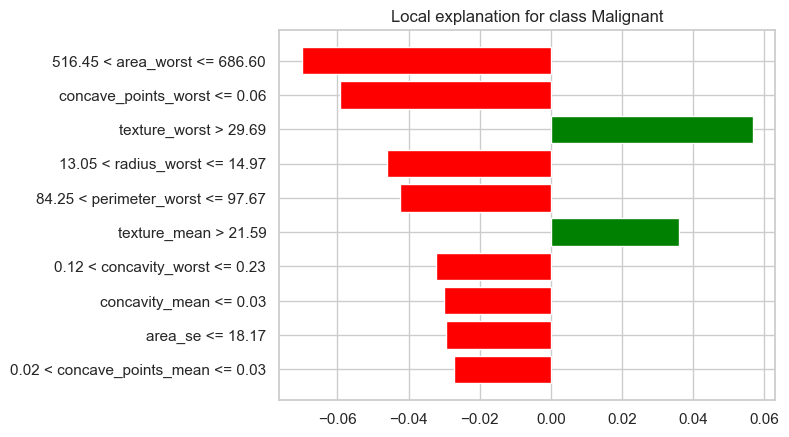
\includegraphics[width=0.8\textwidth]{images/img_2.png}
\caption{Output Image}
\end{figure}

\newpage
\section{نتیجه‌گیری و مقایسه SHAP و LIME}

در این پروژه، ما از مدل Random Forest برای پیش‌بینی سرطان سینه استفاده کردیم و سپس تلاش کردیم تا با استفاده از دو روش SHAP و LIME مدل را تفسیر کنیم.

\subsection{تفاوت SHAP و LIME}

\textbf{LIME (Local Interpretable Model-agnostic Explanations):}
روش LIME سعی می‌کند با تقریب زدن مدل پیچیده اصلی با یک مدل ساده (مثل رگرسیون خطی) در اطراف یک نمونه خاص، رفتار مدل را به صورت محلی توضیح دهد. 
مزیت LIME سرعت بالاتر آن است و اینکه می‌تواند برای هر مدلی استفاده شود. اما مشکل آن این است که توضیحات آن ممکن است ناپایدار باشند (با تغییرات کوچک در نمونه، توضیح تغییر کند).

\textbf{SHAP (SHapley Additive exPlanations):}
روش SHAP بر اساس تئوری بازی‌ها (Game Theory) کار می‌کند و سهم دقیق هر ویژگی را در خروجی نهایی مدل محاسبه می‌کند. 
SHAP از نظر تئوری قوی‌تر و پایدارتر است و توضیحات سراسری (Global) و محلی (Local) منسجم‌تری ارائه می‌دهد. 
اما محاسبه آن، به خصوص برای مدل‌های پیچیده و داده‌های حجیم، بسیار زمان‌برتر از LIME است.

\textbf{نتیجه‌گیری نهایی:}
اگر به دنبال دقت و پایداری درتفسیر هستید، \textbf{SHAP} گزینه بهتری است. اما اگر سرعت اولویت دارد یا نیاز به یک توضیح سریع و تقریبی برای یک نمونه خاص دارید، \textbf{LIME} می‌تواند مفید باشد.

\end{document}